\chapter{PEC1 - Introduction}

This Master's Thesis proposes developing a Geometric Deep Learning architecture conditioned on biological sex for the analysis of spatial transcriptomics (ST) in human atherosclerotic plaques \cite{kanemaru2023spatially, campos2025spatial}. By combining a \textbf{Graph Attention Network (GAT)} with a \textbf{Conditional Multimodal Variational Autoencoder (C-mVAE)}, the model will identify spatially defined cellular niches exhibiting sex-specific transcriptional programs, extracting biomarkers via XAI techniques (GNNExplainer + SHAP) \cite{bronstein2021geometric}. The deliverables include a trained model, a prioritised list of sex-specific biomarkers, and an interactive visualisation application \cite{dong2022deciphering}.

% --- Section 3 ---
\section{Context and justification of work}

Precision medicine relies on capturing not only which genes are expressed, but also the precise spatial and cellular contexts in which their activation occurs. In cardiovascular disease (CVD), the leading cause of mortality among women worldwide \cite{reif2025consideration}, the specific molecular mechanisms governing female vascular tissue remain largely unknown due to historical underrepresentation in clinical trials and functional genomics. 

Standard bioinformatics workflows frequently ignore biological sex or treat it merely as a confounding factor to be removed during batch correction, thereby obscuring sex-specific pathophysiological programs and reducing the efficacy of targeted therapies in women. Addressing this fundamental limitation, a recent review in \textit{Atherosclerosis} (2023) emphasised that \textbf{``future research would require higher inclusion rates of women and well-defined sex-stratified multi-omics analyses``} \cite{hartman2023sex}. 

This project directly responds to this critical gap by introducing an algorithmic solution that incorporates biological sex not as noise, but as an explicit, structural conditioning variable within the neural network architecture which representing a key methodological advancement for the discovery of spatially resolved, sex-specific cardiovascular biomarkers.

\section{Motivation}

The primary motivation stems from the desire to bridge over a decade of professional experience in Machine Learning and MLOps engineering with frontier challenges in bioinformatics and health data science. Academically, this Master's Thesis constitutes a fundamental pillar and an essential proof of concept in preparation for future Ph.D. studies in computational biology or bioinformatics, with a focus on biopharmaceutical applications.

\section{Work objectives}

\begin{itemize}
\item Design and train a Deep Learning architecture (GAT + C-mVAE) for spatial transcriptomics data.
\item Extract sex-specific ligand-receptor communication biomarkers using XAI techniques.
\item Deploy the results in an interactive web application that allows the exploration of cellular niches.
\item In scope: Use of public datasets (GEO), computational deconvolution, and predictive modeling.
\item Out of scope: Collection of in vivo or wet lab clinical samples, experimental clinical validation.
\end{itemize}


\subsection{Main Objective}

The explicit inclusion of biological sex as a conditioning variable in geometric and generative architectures significantly improves the identification and explainability of spatial cellular niches and transcriptomic biomarkers.

\subsection{Research Questions} 

\begin{enumerate}
\item How does the deconvolution of transcriptomic spots using a sex-disaggregated scRNA-seq atlas affect the quality of the initial spatial signal?
\item Is it possible to stabilize the joint training of GNNs and VAEs by introducing Feature-wise Linear Modulation (FiLM) layers conditioned by sex \cite{kipf2016variational}?
\item Which cellular communication axes (ligand-receptor) are prioritized by XAI algorithms \cite{bronstein2021geometric} in female versus male samples?
\end{enumerate}


\section{Focus and method followed}

\begin{description}
\item[Research strategy:] 
A quantitative and experimental research strategy will be adopted, evaluating algorithmic performance against baseline models (such as STAGATE \cite{dong2022deciphering}) using established metrics (ARI, NMI).
\end{description}

\begin{description}
\item[Development methodology:] 
An iterative approach based on prototyping will be used, implementing reproducible Machine Learning operations (MLOps) pipelines \cite{long2023spatially}.
\end{description}

\begin{description}
\item[Tools:] 
PyTorch Geometric (network architecture), Squidpy and Scanpy \cite{slenders2024single} (spatial and scRNA-seq processing), GitHub (version control), Docker (isolated environments), and Streamlit or R Shiny (final dashboard creation).
\end{description}

\section{Impact on sustainability, ethics-social and diversity}
\label{s:etic}

The scientific core of this project is, by definition, the integration of the gender perspective and biological sex into precision medicine, seeking to correct the biases of generic models. Additionally:

\begin{enumerate}
\item SAGER (Sex and Gender Equity in Research) guidelines \cite{heidari2016sex} will be applied for the correct reporting of variables in the analyses.
\item All technical documentation and the final report will use inclusive and non-sexist language.
\item The visualization dashboard will be designed and tested to ensure that differences in results across various biological profiles are presented clearly and without presentation biases.
\end{enumerate}

% --- Section 7 ---
\section{Methodological Design and Consistency}

\subsection{Pipeline Overview}

\begin{table}[htbp]
\centering
\small
\begin{tabularx}{\textwidth}{c l X X X}
\toprule
\textbf{Phase} & \textbf{Name} & \textbf{Selected Method} & \textbf{Considered Alternative} & \textbf{Selection Criteria} \\
\midrule
1 & Ingestion \& QC & SpaceRanger + Squidpy & STARsolo, Cellranger & GEO compatibility, documentation \\
2 & Deconvolution & SPOTlight (scRNA GSE210572) & RCTD, CARD & Sex-stratified ref. available \cite{elosua2021spotlight} \\
3 & Baseline GNN & STAGATE (GAT) & SpaGCN \cite{hu2021spagcn}, BayesSpace & Top ARI performance in benchmarks \cite{dong2022deciphering, hu2021spagcn} \\
4 & Sex-Strat. GNN & PyTorch Geometric + FiLM & Original Proposal & Literature gap verified \\
5 & Integration & MOFA+ $\rightarrow$ C-mVAE PoE & DIABLO, scVI & MOFA+ validated in CVD \cite{argelaguet2020mofa} \\
6 & XAI \& Viz. & GNNExplainer + SHAP + Streamlit & LIME, IntegratedGrad \cite{bronstein2021geometric} & Native graph support \\
\bottomrule
\end{tabularx}
\end{table}



% -- Dataset used ---
\subsection{Datasets Used}

\begin{table}[htbp]
\centering
\small
\begin{tabularx}{\textwidth}{l l l X}
\toprule
\textbf{Dataset} & \textbf{Source} & \textbf{Access} & \textbf{Role in the Model} \\
\midrule
GEO GSE233025 & Campos et al. (2025) \cite{campos2025spatial} & Open, Immediate & Expression matrix ($\mathbf{X}$) + Spatial coordinates ($\mathbf{A}$) \\
HCA Heart (Visium) & Human Cell Atlas \cite{kanemaru2023spatially} & Open (CZI) & Cross-validation \\
GEO GSE210572 & Sukhavasi et al. (2025) \cite{sukhavasi2025single} & Open, Immediate & Sex-stratified scRNA-seq reference \\
GTEx v10 & GTEx Portal & Open & Epigenomic layer \cite{argelaguet2020mofa} for C-mVAE \\
\bottomrule
\end{tabularx}
\end{table}

% --- Section 8 ---
\newpage
\section{Study Limitations}
\begin{itemize}[leftmargin=*]
    \item \textbf{Snapshot Bias:} ST data represents a static physiological state; cell interactions reflect spatial proximity rather than dynamic causality \cite{slenders2024single}.
    \item \textbf{Visium Resolution (55 $\mu$m):} Dependence on SPOTlight deconvolution accuracy in the absence of subcellular CosMx resolution data \cite{elosua2021spotlight}.
    \item \textbf{Sample Imbalance:} Potential sex imbalance in public datasets, explicitly documented following SAGER standards \cite{heidari2016sex}.
    \item \textbf{Lack of Wet-Lab Validation:} Experimental validation (qPCR/IHC) remains out of scope for this computational thesis \cite{hartman2023sex}.
    \item \textbf{Over-smoothing:} Risk inherent to deep GNNs, mitigated via skip connections \cite{hu2021spagcn}.
\end{itemize}

% --- Section 10 ---
\newpage
\section{Feasibility}

\subsection{Data Access}
All primary datasets are publicly available with immediate, unrestricted access (GEO, Human Cell Atlas, GTEx) \cite{campos2025spatial, sukhavasi2025single, kanemaru2023spatially} 

\subsection{Identification of the SDGs}

\begin{description}
\item[SDG 3] s
(Good Health and Well-being): By advancing analytical techniques for precision medicine and the early identification of biomarkers in complex diseases.
\end{description}

\begin{description}
\item[SDG 5] 
(Gender Equality): By developing algorithms that correct historical biases in medical data through stratified and conditioned architectures.
\end{description}

\begin{description}
\item[SDG 9] 
(Industry, Innovation and Infrastructure): Providing technological innovation through the use of explainable artificial intelligence (XAI) in bioinformatics infrastructures..
\end{description}

% --- Section 14 ---
\section{Plagiarism Prevention}
The document will be processed through UOC/UB anti-plagiarism screening (Turnitin). Code will be released under the open-source MIT License on GitHub. References follow APA 7th style.


% ??? RISK ANALYSIS ????????????????????????????????????????????????????????????
\section{Risk Analysis and Mitigation}
\label{s:risks}

The following table identifies the principal risks associated with the research,
their likelihood and impact, and the corresponding mitigation strategies.

\begin{table}[htbp]
\centering
\small
\caption{Risk register and mitigation plan for SexOmics-Spatial TFM}
\label{tab:risks}
\begin{tabularx}{\textwidth}{l c c X}
\toprule
\textbf{Risk} & \textbf{Likelihood} & \textbf{Impact} & \textbf{Mitigation Strategy} \\
\midrule
Joint GNN+VAE training divergence &
Medium & High &
Decouple training: first optimise VAE embeddings; use them as static node features
for the GNN in a second stage \cite{kipf2016variational}. \\
\addlinespace
Visium resolution insufficient for\\sex-specific niche detection &
Low & High &
Switch to CosMx single-transcript data from Campos et al.\ \cite{campos2025spatial},
which provides subcellular resolution without deconvolution. \\
\addlinespace
Sex imbalance in public datasets &
Medium & Medium &
Apply inverse class weighting during training; report imbalance explicitly
following SAGER guidelines \cite{heidari2016sex}. \\
\addlinespace
CosMx data not available in GEO\\at project start &
Low & Medium &
Fall back exclusively to Visium + SPOTlight deconvolution \cite{elosua2021spotlight}
using GSE210572 as sex-stratified reference. \\
\addlinespace
Over-smoothing in deep GNN layers &
Medium & Medium &
Introduce skip connections and limit architecture to 3 GAT layers;
validated in ST benchmarks \cite{dong2022deciphering}. \\
\addlinespace
GPU compute cost exceeds budget &
Low & Low &
Use Kaggle Notebooks (30 h GPU/week, free) as primary alternative to
Google Colab Pro; apply NeighborLoader subsampling in PyTorch Geometric. \\
\addlinespace
Physical tissue discontinuity (necrosis,\\calcification artefacts) &
Low & Medium &
Replace standard edge-loss with a Gromov--Wasserstein optimal transport
cost function for topological alignment across tissue gaps. \\
\bottomrule
\end{tabularx}
\end{table}

\newpage
\section{Work schedule}

Below is the detailed Gantt chart covering all project milestones.

{\small
\begin{xltabular}{\linewidth}{c >{\raggedright\arraybackslash}p{2.8cm} >{\raggedright\arraybackslash}X c c c c c}
\caption{Master's Thesis Work Breakdown Structure (WBS) \& Effort Estimates}
\label{tab:tfm_wbs}\\
\toprule
\textbf{ID} & \textbf{Phase / Deliverable} & \textbf{Task Description} & \textbf{Start Date} & \textbf{End Date} & \textbf{Days} & \textbf{Hours} & \textbf{Dep.} \\
\midrule
\endfirsthead

\multicolumn{8}{l}{\small\textit{(continued from Table~\thetable)}} \\
\toprule
\textbf{ID} & \textbf{Phase / Deliverable} & \textbf{Task Description} & \textbf{Start Date} & \textbf{End Date} & \textbf{Days} & \textbf{Hours} & \textbf{Dep.} \\
\midrule
\endhead

\midrule
\multicolumn{8}{r}{\small\textit{continued on next page\ldots}} \\
\endfoot

\midrule
\multicolumn{5}{r}{\textbf{Total Workload Estimate:}} & \textbf{113} & \textbf{367} & \\
\bottomrule
\endlastfoot

1.1 & PEC 1: Work Plan & Define Title, Keywords \& Proposal Summary & 2026-09-23 & 2026-09-26 & 4 & 12 & -- \\
1.2 & PEC 1: Work Plan & Context, Justification \& Motivation & 2026-09-27 & 2026-09-29 & 3 & 10 & 1.1 \\
1.3 & PEC 1: Work Plan & Define General/Specific Objectives, Main Hypothesis \& Research Questions & 2026-09-30 & 2026-10-02 & 3 & 10 & 1.2 \\
1.4 & PEC 1: Work Plan & Research Strategy, Gender Perspective \& SDGs Alignment & 2026-10-03 & 2026-10-05 & 3 & 12 & 1.3 \\
1.5 & PEC 1: Work Plan & Work Plan Schedule, Risk Analysis \& Final Delivery (PEC 1 Submission) & 2026-10-06 & 2026-10-07 & 2 & 8 & 1.4 \\
2.1 & PEC 2: State of the Art & Systematic Literature Search (Scopus, Web of Science, PubMed) & 2026-10-08 & 2026-10-15 & 8 & 25 & 1.5 \\
2.2 & PEC 2: State of the Art & Download Spatial Transcriptomics \& scRNA-seq Datasets (GEO) + QC & 2026-10-16 & 2026-10-22 & 7 & 20 & 2.1 \\
2.3 & PEC 2: State of the Art & Synthesis of Benchmark Methods \& Critical Review & 2026-10-23 & 2026-10-29 & 7 & 20 & 2.1 \\
2.4 & PEC 2: State of the Art & Cellular Deconvolution Baseline Execution \& Progress Report (PEC 2 Submission) & 2026-10-30 & 2026-11-04 & 6 & 15 & 2.2, 2.3 \\
3.1 & PEC 3: Implementation & GNN Architecture Design \& Spatial Graph Construction (PyTorch Geometric) & 2026-11-05 & 2026-11-12 & 8 & 30 & 2.4 \\
3.2 & PEC 3: Implementation & Biological Sex-Conditioned VAE Integration (FiLM layers) & 2026-11-13 & 2026-11-20 & 8 & 30 & 3.1 \\
3.3 & PEC 3: Implementation & XAI Biomarker Extraction \& Algorithmic Validation & 2026-11-21 & 2026-11-27 & 7 & 25 & 3.2 \\
3.4 & PEC 3: Implementation & Interactive Visualization Dashboard \& Implementation Report (PEC 3 Submission) & 2026-11-28 & 2026-12-02 & 5 & 20 & 3.3 \\
4.1 & PEC 4: Final Report & Structure Master Thesis Report \& Write Introduction/Background & 2026-12-03 & 2026-12-10 & 8 & 25 & 3.4 \\
4.2 & PEC 4: Final Report & Compile Experimental Results, Figures \& Discussion Synthesis & 2026-12-11 & 2026-12-20 & 10 & 35 & 4.1 \\
4.3 & PEC 4: Final Report & Formal Evaluation of Ethics, SDGs \& Gender Impact Integration & 2026-12-21 & 2026-12-28 & 8 & 20 & 4.2 \\
4.4 & PEC 4: Final Report & Final Document Formatting (\textless 90 pages), References Audit \& PDF Delivery (PEC 4 Submission) & 2026-12-29 & 2027-01-07 & 10 & 25 & 4.3 \\
5.1 & PEC 5: Presentation & Virtual Slide Deck Design (Max 20 slides, UOC Official Template) & 2027-01-08 & 2027-01-10 & 3 & 12 & 4.4 \\
5.2 & PEC 5: Presentation & Oral Defense Rehearsal \& Video Recording (\textless 20 minutes limit) & 2027-01-11 & 2027-01-12 & 2 & 10 & 5.1 \\
5.3 & PEC 5: Presentation & Defense Submission (Video File \& Presentation Deck Delivery) & 2027-01-13 & 2027-01-13 & 1 & 3 & 5.2 \\
\end{xltabular}
}

% Comienza la p�gina en formato landscape

\newpage
\begin{landscape}
\begin{figure}[htbp]
    \centering
    % Como declaramos \graphicspath{{images/}}, solo pones el nombre del archivo:
    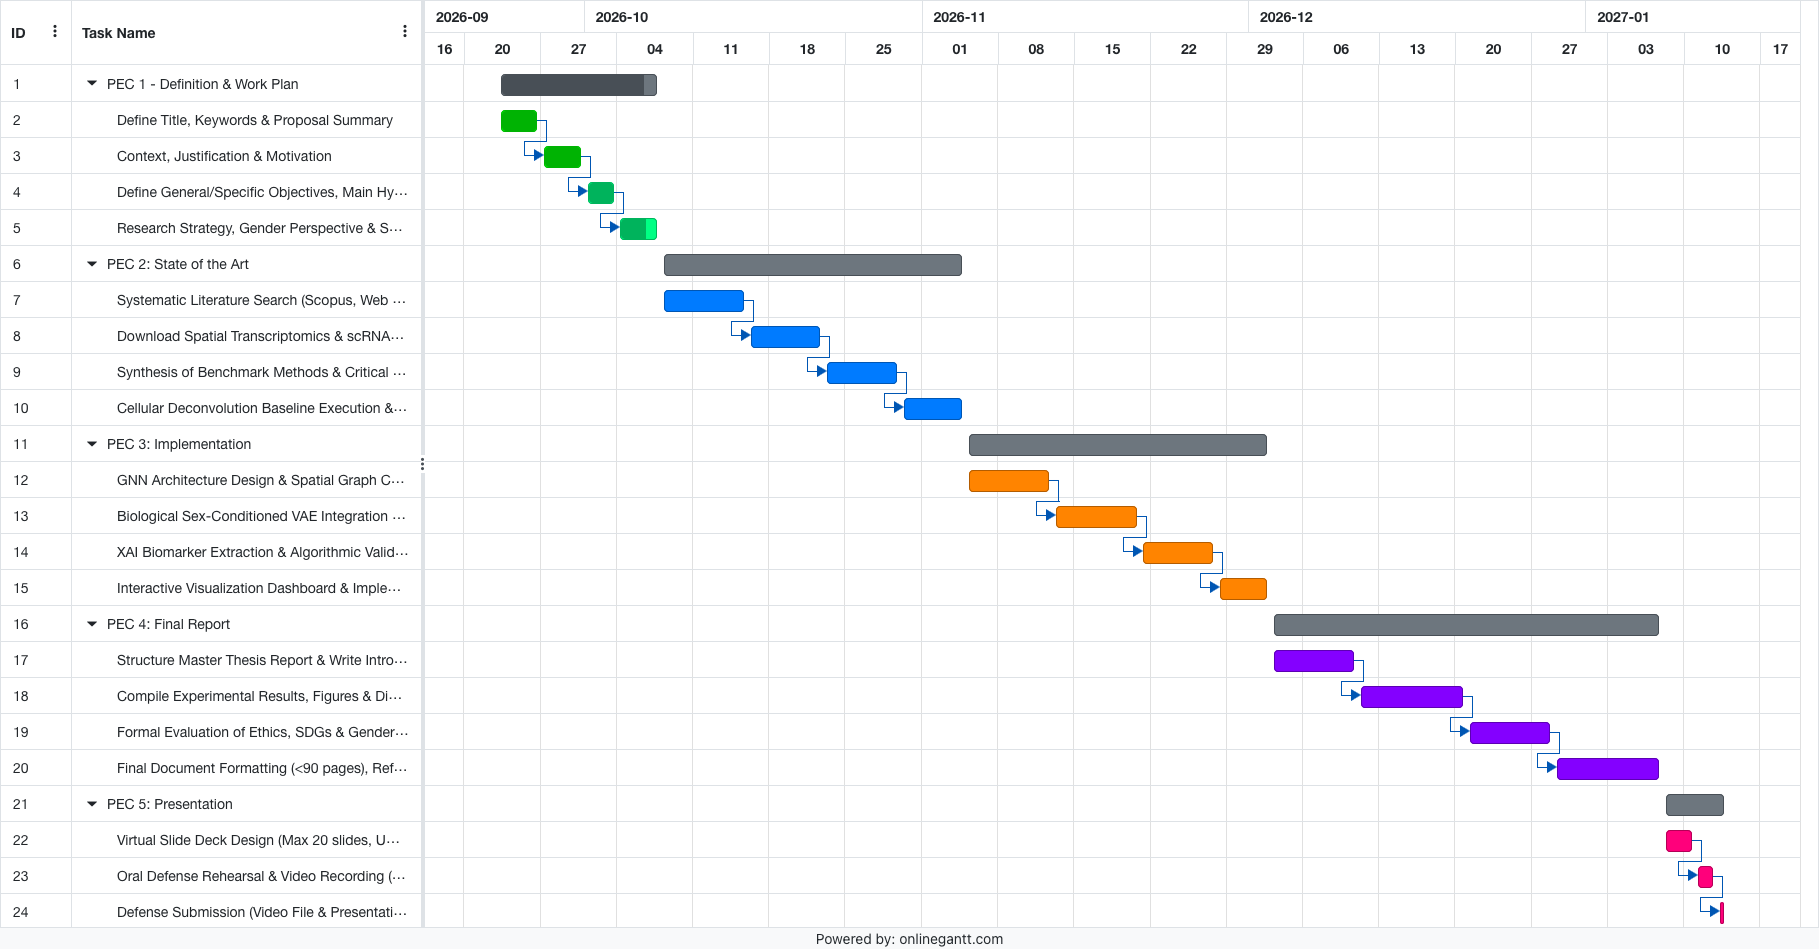
\includegraphics[width=0.9\linewidth]{Online Gantt 20261002.png}
    \caption{Master's Thesis Schedule and Work Breakdown Structure.}
    \label{fig:gantt_schedule}
\end{figure}
\end{landscape}


\begin{figure}[htbp]
\begin{center}

\end{center}
\end{figure}